\documentclass[specialist,
substylefile = spbu_report.rtx,
subf,href,colorlinks=true, 12pt]{disser}

\usepackage[T2A]{fontenc}
\usepackage[utf8]{inputenc}
\usepackage[english,russian]{babel}

\usepackage[a4paper,
mag=1000, includefoot,
left=3cm, right=1.5cm, top=2cm, bottom=2cm, headsep=1cm, footskip=1cm]{geometry}

\usepackage{graphicx,subcaption,ragged2e}

\usepackage{booktabs}

\usepackage{amsthm}
\usepackage{amsmath}
\usepackage{amssymb}
\usepackage{hhline}
\usepackage{xcolor}
\usepackage{array}
\usepackage{bbm}
\usepackage{bm}

\theoremstyle{definition}
\newtheorem{definition}{Определение}[section]
\newtheorem{algorithm}{Алгоритм}
\newtheorem{remark}{Замечание}[section]
\newtheorem{example}{Пример}[section]
\newtheorem{assumption}{Предположение}[section]
\newtheorem{statement}{Утверждение}
\newtheorem{proposition}{Предложение}[section]
\newtheorem{corollary}{Следствие}[section]

\newcommand{\R}{\mathbb{R}}
\newcommand{\Z}{\mathbb{Z}}
\newcommand{\const}{\mathrm{const}}
\newcommand{\im}{\mathrm{i}}

\usepackage{float}

\usepackage{rotating}

%new calligraphic font for subspaces 
\usepackage{euscript}
\newcommand{\cA}{\EuScript{A}}
\newcommand{\cB}{\EuScript{B}}
\newcommand{\cC}{\EuScript{C}}
\newcommand{\cD}{\EuScript{D}}
\newcommand{\cE}{\EuScript{E}}
\newcommand{\cF}{\EuScript{F}}
\newcommand{\cG}{\EuScript{G}}
\newcommand{\cH}{\EuScript{H}}
\newcommand{\cI}{\EuScript{I}}
\newcommand{\cJ}{\EuScript{J}}
\newcommand{\cK}{\EuScript{K}}
\newcommand{\cL}{\EuScript{L}}
\newcommand{\cM}{\EuScript{M}}
\newcommand{\cN}{\EuScript{N}}
\newcommand{\cO}{\EuScript{O}}
\newcommand{\cP}{\EuScript{P}}
\newcommand{\cQ}{\EuScript{Q}}
\newcommand{\cR}{\EuScript{R}}
\newcommand{\cS}{\EuScript{S}}
\newcommand{\cT}{\EuScript{T}}
\newcommand{\cU}{\EuScript{U}}
\newcommand{\cV}{\EuScript{V}}
\newcommand{\cW}{\EuScript{W}}
\newcommand{\cX}{\EuScript{X}}
\newcommand{\cY}{\EuScript{Y}}
\newcommand{\cZ}{\EuScript{Z}}

%font for text indices like transposition X^\mathrm{T}
\newcommand{\rmA}{\mathrm{A}}
\newcommand{\rmB}{\mathrm{B}}
\newcommand{\rmC}{\mathrm{C}}
\newcommand{\rmD}{\mathrm{D}}
\newcommand{\rmE}{\mathrm{E}}
\newcommand{\rmF}{\mathrm{F}}
\newcommand{\rmG}{\mathrm{G}}
\newcommand{\rmH}{\mathrm{H}}
\newcommand{\rmI}{\mathrm{I}}
\newcommand{\rmJ}{\mathrm{J}}
\newcommand{\rmK}{\mathrm{K}}
\newcommand{\rmL}{\mathrm{L}}
\newcommand{\rmM}{\mathrm{M}}
\newcommand{\rmN}{\mathrm{N}}
\newcommand{\rmO}{\mathrm{O}}
\newcommand{\rmP}{\mathrm{P}}
\newcommand{\rmQ}{\mathrm{Q}}
\newcommand{\rmR}{\mathrm{R}}
\newcommand{\rmS}{\mathrm{S}}
\newcommand{\rmT}{\mathrm{T}}
\newcommand{\rmU}{\mathrm{U}}
\newcommand{\rmV}{\mathrm{V}}
\newcommand{\rmW}{\mathrm{W}}
\newcommand{\rmX}{\mathrm{X}}
\newcommand{\rmY}{\mathrm{Y}}
\newcommand{\rmZ}{\mathrm{Z}}

%tt font for time series
\newcommand{\tA}{\mathsf{A}}
\newcommand{\tB}{\mathsf{B}}
\newcommand{\tC}{\mathsf{C}}
\newcommand{\tD}{\mathsf{D}}
\newcommand{\tE}{\mathsf{E}}
\newcommand{\tF}{\mathsf{F}}
\newcommand{\tG}{\mathsf{G}}
\newcommand{\tH}{\mathsf{H}}
\newcommand{\tI}{\mathsf{I}}
\newcommand{\tJ}{\mathsf{J}}
\newcommand{\tK}{\mathsf{K}}
\newcommand{\tL}{\mathsf{L}}
\newcommand{\tM}{\mathsf{M}}
\newcommand{\tN}{\mathsf{N}}
\newcommand{\tO}{\mathsf{O}}
\newcommand{\tP}{\mathsf{P}}
\newcommand{\tQ}{\mathsf{Q}}
\newcommand{\tR}{\mathsf{R}}
\newcommand{\tS}{\mathsf{S}}
\newcommand{\tT}{\mathsf{T}}
\newcommand{\tU}{\mathsf{U}}
\newcommand{\tV}{\mathsf{V}}
\newcommand{\tW}{\mathsf{W}}
\newcommand{\tX}{\mathsf{X}}
\newcommand{\tY}{\mathsf{Y}}
\newcommand{\tZ}{\mathsf{Z}}

%bf font for matrices
\newcommand{\bfA}{\mathbf{A}}
\newcommand{\bfB}{\mathbf{B}}
\newcommand{\bfC}{\mathbf{C}}
\newcommand{\bfD}{\mathbf{D}}
\newcommand{\bfE}{\mathbf{E}}
\newcommand{\bfF}{\mathbf{F}}
\newcommand{\bfG}{\mathbf{G}}
\newcommand{\bfH}{\mathbf{H}}
\newcommand{\bfI}{\mathbf{I}}
\newcommand{\bfJ}{\mathbf{J}}
\newcommand{\bfK}{\mathbf{K}}
\newcommand{\bfL}{\mathbf{L}}
\newcommand{\bfM}{\mathbf{M}}
\newcommand{\bfN}{\mathbf{N}}
\newcommand{\bfO}{\mathbf{O}}
\newcommand{\bfP}{\mathbf{P}}
\newcommand{\bfQ}{\mathbf{Q}}
\newcommand{\bfR}{\mathbf{R}}
\newcommand{\bfS}{\mathbf{S}}
\newcommand{\bfT}{\mathbf{T}}
\newcommand{\bfU}{\mathbf{U}}
\newcommand{\bfV}{\mathbf{V}}
\newcommand{\bfW}{\mathbf{W}}
\newcommand{\bfX}{\mathbf{X}}
\newcommand{\bfY}{\mathbf{Y}}
\newcommand{\bfZ}{\mathbf{Z}}

%bb font for standard spaces and expectation
\newcommand{\bbA}{\mathbb{A}}
\newcommand{\bbB}{\mathbb{B}}
\newcommand{\bbC}{\mathbb{C}}
\newcommand{\bbD}{\mathbb{D}}
\newcommand{\bbE}{\mathbb{E}}
\newcommand{\bbF}{\mathbb{F}}
\newcommand{\bbG}{\mathbb{G}}
\newcommand{\bbH}{\mathbb{H}}
\newcommand{\bbI}{\mathbb{I}}
\newcommand{\bbJ}{\mathbb{J}}
\newcommand{\bbK}{\mathbb{K}}
\newcommand{\bbL}{\mathbb{L}}
\newcommand{\bbM}{\mathbb{M}}
\newcommand{\bbN}{\mathbb{N}}
\newcommand{\bbO}{\mathbb{O}}
\newcommand{\bbP}{\mathbb{P}}
\newcommand{\bbQ}{\mathbb{Q}}
\newcommand{\bbR}{\mathbb{R}}
\newcommand{\bbS}{\mathbb{S}}
\newcommand{\bbT}{\mathbb{T}}
\newcommand{\bbU}{\mathbb{U}}
\newcommand{\bbV}{\mathbb{V}}
\newcommand{\bbW}{\mathbb{W}}
\newcommand{\bbX}{\mathbb{X}}
\newcommand{\bbY}{\mathbb{Y}}
\newcommand{\bbZ}{\mathbb{Z}}

%got font for any case
\newcommand{\gA}{\mathfrak{A}}
\newcommand{\gB}{\mathfrak{B}}
\newcommand{\gC}{\mathfrak{C}}
\newcommand{\gD}{\mathfrak{D}}
\newcommand{\gE}{\mathfrak{E}}
\newcommand{\gF}{\mathfrak{F}}
\newcommand{\gG}{\mathfrak{G}}
\newcommand{\gH}{\mathfrak{H}}
\newcommand{\gI}{\mathfrak{I}}
\newcommand{\gJ}{\mathfrak{J}}
\newcommand{\gK}{\mathfrak{K}}
\newcommand{\gL}{\mathfrak{L}}
\newcommand{\gM}{\mathfrak{M}}
\newcommand{\gN}{\mathfrak{N}}
\newcommand{\gO}{\mathfrak{O}}
\newcommand{\gP}{\mathfrak{P}}
\newcommand{\gQ}{\mathfrak{Q}}
\newcommand{\gR}{\mathfrak{R}}
\newcommand{\gS}{\mathfrak{S}}
\newcommand{\gT}{\mathfrak{T}}
\newcommand{\gU}{\mathfrak{U}}
\newcommand{\gV}{\mathfrak{V}}
\newcommand{\gW}{\mathfrak{W}}
\newcommand{\gX}{\mathfrak{X}}
\newcommand{\gY}{\mathfrak{Y}}
\newcommand{\gZ}{\mathfrak{Z}}

%old calligraphic font
\newcommand{\calA}{\mathcal{A}}
\newcommand{\calB}{\mathcal{B}}
\newcommand{\calC}{\mathcal{C}}
\newcommand{\calD}{\mathcal{D}}
\newcommand{\calE}{\mathcal{E}}
\newcommand{\calF}{\mathcal{F}}
\newcommand{\calG}{\mathcal{G}}
\newcommand{\calH}{\mathcal{H}}
\newcommand{\calI}{\mathcal{I}}
\newcommand{\calJ}{\mathcal{J}}
\newcommand{\calK}{\mathcal{K}}
\newcommand{\calL}{\mathcal{L}}
\newcommand{\calM}{\mathcal{M}}
\newcommand{\calN}{\mathcal{N}}
\newcommand{\calO}{\mathcal{O}}
\newcommand{\calP}{\mathcal{P}}
\newcommand{\calQ}{\mathcal{Q}}
\newcommand{\calR}{\mathcal{R}}
\newcommand{\calS}{\mathcal{S}}
\newcommand{\calT}{\mathcal{T}}
\newcommand{\calU}{\mathcal{U}}
\newcommand{\calV}{\mathcal{V}}
\newcommand{\calW}{\mathcal{W}}
\newcommand{\calX}{\mathcal{X}}
\newcommand{\calY}{\mathcal{Y}}
\newcommand{\calZ}{\mathcal{Z}}


\setcounter{tocdepth}{2}

\begin{document}
\section{Вспомогательные определения}
В данном разделе введем некоторые обозначения, которые будем использовать в дальнейшем.
\begin{definition}\label{def:stationary}
	Случайный процесс $\{Y_t:t\in\Z\}$ называют стационарным (в широком смысле), если
	\begin{enumerate}
		\item $\mathsf{E}Y_t\equiv\const$ (среднее постоянно по времени);
		\item $\mathsf{cov}(Y_t,Y_{t+h})=\gamma(h)$ (ковариация зависит только от лага $h$).
	\end{enumerate}
\end{definition}
\begin{remark}
	Поскольку $\gamma(0)=\mathsf{cov}(Y_t,Y_t)=\mathsf{D}Y_t$, то дисперсия также не меняется со временем.
\end{remark}
\begin{remark}
	Далее под стационарностью будет подразумеваться именно стационарность в широком смысле.
\end{remark}
\begin{definition}
	Случайный процесс $\{\varepsilon_t\}$ называют белым шумом $\mathrm{WN}(0, \sigma^2)$, если он стационарный, $\mathsf{E}\varepsilon_t=0$, $\gamma(h)=0$ $\forall h\ne 0$ и $\mathsf{D}\varepsilon_t=\sigma^2$.
\end{definition}

\begin{definition}
	Моделью $\mathrm{ARMA}(p, q)$, где $p$, $q\in \mathbb{N}\cup\{0\}$ называют случайный процесс $\{X_t\}$, удовлетворяющий соотношению
	\[
	X_t=\varepsilon_t + \sum_{i=1}^p \phi_i X_{t-i} + \sum_{i=1}^q\theta_i\varepsilon_{t-i},
	\]
	где $\{\varepsilon_t\}\sim\mathrm{WN}(0, \sigma^2)$.
\end{definition}

\begin{definition}
	Спектральной плотностью стационарного процесса называется такая функция $f(\omega)$, что
	\[
		\gamma(h)=2\int_{0}^{1/2} e^{2\pi h\omega\im}f(\omega)d\omega.
	\]
\end{definition}
\begin{definition}
	Пусть $\{Y_t\}$ --- cтационарный процесс. Функцию
	\[
		I(\omega)=\frac1n\left|\sum_{j=1}^{n} Y_je^{-2\pi \omega j\mathrm{i}}\right|^2
	\]
	называют периодограммой выборки размера $n$ процесса $\{Y_t\}$.
\end{definition}


\section{Процессы с длинной памятью}

\begin{definition}\label{def:longmemory}
	Говорят, что стационарный процесс $\{Y_t\}$ обладает длинной памятью, если
	\[
		\sum_{h=0}^H|\gamma(h)|\to\infty,
	\]
	при $H\to\infty$. Иначе говорят, что $\{Y_t\}$ обладает короткой памятью:
	\[
		\sum_{h=0}^\infty|\gamma(h)|<\infty.
	\]
\end{definition}
Существуют и альтернативные определения процессов с длинной памятью, которые можно найти в~\cite[Section 3.1]{Palma2006}. Там же показано, что они согласованы с определением~\ref{def:longmemory}.
% \begin{enumerate}
%     \item Процесс с длинной памятью можно определить как процесс с гиперболическим затуханием автоковариационной функции:
%     \[
%     \gamma(h)\sim h^{2d-1}\ell_1(h),
%     \]
%     при $h\to \infty$, где $d$ так называемый параметр длинной памяти и $\ell_1(\cdot)$ --- медленно меняющаяся на бесконечности функция.
%     \item Также его можно определить поведением спектральной плотности в окрестности нуля:
%     \[
%     f(\lambda)\sim|\lambda|^{-2d}\ell_2(1/|\lambda|),
%     \]
%     при $\lambda\to0$, где $\ell_2(\cdot)$ --- медленно меняющаяся на бесконечности функция.
% \end{enumerate}
\begin{example}
	Процессом с короткой памятью является, например, стационарная модель $\mathrm{ARMA}(p, q)$, поскольку $|\gamma(h)|\leqslant CR^h$, где $C>0$ и $0<R<1$~\cite{BoxJenkins2016}.
\end{example}
% Примером стационарного процесса с длинной памятью является дробно интегрированный процесс.
Введем понятие дробного интегрирования $(1-L)^d$, где $L$ --- оператор сдвига. Например, для $d=1$ имеем $(1-L)Y_t=Y_t-Y_{t-1}$, для $d=2$ --- $(1-L)^2Y_t=Y_t-2Y_{t-1}+Y_{t-2}$, и так далее. Обобщим этот оператор для нецелых $d$ с помощью разложения в ряд Тейлора функции $(1-x)^d$ в нуле:
\[
	\begin{aligned}
		(1-x)^d & =1-dx-\frac{d(1-d)}{2}x^2-\frac{d(1-d)(2-d)}{3!}x^3-\ldots             \\
		        & =\sum_{j=0}^\infty \pi_j(d)x^j=\sum_{j=0}^\infty\binom{d}{j}(-1)^jx^j,
	\end{aligned}
\]
где $\binom{d}{j}$ --- обобщенный биномиальный коэффициент. Коэффиенты $\pi_j(d)$ удовлетворяют соотношению
\begin{equation}\label{eq:pi_j}
	\pi_j(d)=(-1)^j\binom{d}{j}=\frac{j-1-d}{j}\pi_{j-1}(d)=\frac{\Gamma(j-d)}{\Gamma(j+1)\Gamma(-d)},
\end{equation}
где $\Gamma(x)$ --- гамма функция. Заметим, что второе равенство в формуле~\eqref{eq:pi_j} верно для любых $d$, третье же верно только для $d\not\in\bbN\cup\{0\}$, поскольку гамма функция не определена для неположительных целых чисел.
% \begin{assumption}\label{as1}
% 	Пусть $\{X_t\}$ представляет собой $\mathrm{MA}(\infty)$ процесс,
% 	\[
% 		X_t=\sum_{j=0}^\infty c_j\varepsilon_{t-j},\quad \{\varepsilon_t\}\sim \mathrm{WN}(0, \sigma^2),
% 	\]
% 	который абсолютно суммируемый, $\sum_{j=0}^\infty |c_j|<\infty$, и $\sum_{j=0}^\infty c_j\ne0$.
% \end{assumption}
% \begin{remark}
%     Данное условие равносильно тому, что $0<f_X(0)<\infty$.
% \end{remark}
\begin{definition}\label{def:arfima}
	Пусть процесс $\{Y_t\}$ определен соотношением
	\[
		\begin{aligned}
			Y_t=(1-L)^{-d}X_t=\sum_{k=0}^\infty \pi_k(-d)X_{t-k}
		\end{aligned},\quad d<1/2,
	\]
	где $\pi_k(-d)$ из формулы~\eqref{eq:pi_j}, $\{X_t\}$ --- стационарная и обратимая модель $\mathrm{ARMA}(p, d)$. Процесс $\{Y_t\}$ называют дробно интегрированной моделью $\mathrm{ARMA}$ или $\mathrm{ARFIMA}(p, d, q)$.
\end{definition}
% \begin{remark}
% 	При $p=q=0$ процесс $\{X_t\}$ из определения~\ref{def:arfima} является белым шумом. В таком случае процесс $\{Y_t\}$ называют дробно интегрированным шумом или $\mathrm{FIN}(d)$.
% \end{remark}

\begin{proposition}\label{prop1}
	$\mathrm{ARFIMA}(p, d, q)$ является стационарным процессом с нулевым средним при $d<1/2$. Его спектральная плотность определяется выражением
	\begin{equation}\label{eq:spec_long}
		\begin{aligned}
			f(\omega) & =\sigma^2 4^{-d}\sin^{-2d}\left(\pi\omega\right)\frac{\left|\theta(e^{-2\pi \omega\im})\right|^2}{\left|\phi(e^{-2\pi\omega\im})\right|^2},\quad\omega>0\\
			&\sim\sigma^2\omega^{-2d}\frac{|\theta(1)|^2}{|\phi(1)|^2},\quad \omega\to0,
		\end{aligned}
	\end{equation}
\end{proposition}
\begin{proof}
	См.~\cite[Proposition 6.1]{Hassler2018}.
\end{proof}
\begin{remark}
	Из формулы~\eqref{eq:spec_long} видно, что спектральная плотность дробно интегрированного процесса монотонно убывает (возрастает) тогда и только тогда, когда монотонно убывает (возрастает) спектральная плотность процесса $\{X_t\}$.
\end{remark}
\begin{corollary}\label{corollary1}
	В условиях предложения~\ref{prop1} при $0<d<1/2$
	\[
		\gamma(h)\sim C_{\gamma,d}h^{2d-1},\quad h\to\infty,
	\]
	где
	\[
		C_{\gamma,d}=\sigma^2 \frac{|\theta(1)|^2}{|\phi(1)|^2} \frac{\Gamma(1-2d)}{\Gamma(d)\Gamma(1-d)}.
	\]
\end{corollary}
\begin{proof}
	См.~\cite[Corollary 6.1]{Hassler2018}.
\end{proof}
\begin{remark}
	Из следствия~\ref{corollary1} сразу следует, что $\mathrm{ARFIMA}(p, d, q)$ с $d\in(0, 1/2)$ обладает длинной памятью.
\end{remark}
% \begin{example}
% 	Если $\{X_t\}$ является белым шумом $\mathrm{WN}(0, \sigma^2)$, то $\{Y_t\}$ называют дробно интегрированным шумом ($\mathrm{FIN}$). Его спектральная плотность имеет вид
% 	\[
% 		f_Y(\omega)=\sigma^2 4^{-d}\sin^{-2d}\left(\pi\omega\right).
% 	\]
% 	Отсюда следует, что дробно интегрированный шум всегда обладает монотонной спектральной плотностью.
% \end{example}
% \begin{example}
% 	Стационарный и обратимый $\mathrm{ARMA}$ процесс удовлетворяют предположениям о $\{X_t\}$ в определении~\ref{def:FI}~\cite[Proposition 3.5]{Hassler2018}. Процесс $\{Y_t\}$ в таком случае называют дробно интегрированным $\mathrm{ARMA}$ процессом или коротко $\mathrm{ARFIMA}(p, d, q)$. Его спектральная плотность имеет вид
% 	\[
% 		f_Y(\omega)=\sigma^2 4^{-d}\sin^{-2d}\left(\pi\omega\right)\frac{\left|\theta(e^{-2\pi \omega\im})\right|^2}{\left|\phi(e^{-2\pi\omega\im})\right|^2},
% 	\]
% 	где $\phi$ и $\theta$ --- характеристические полиномы $\mathrm{AR}$ и $\mathrm{MA}$ частей $\mathrm{ARMA}$ соответственно.
% \end{example}

\subsection{Возникновение процессов с длинной памятью}
Нас интересуют процессы с монотонной спектральной плотностью, поскольку они довольно распространены в реальном мире. Такими процессами являются процессы со степенной спектральной плотностью $f(\omega)\sim \omega^{-\alpha}$, имеющие большое применение в различных областях, например, в физике, биологии, астрофизике, геофизике и экономике.

Процессы с длинной памятью, являющиеся частным случаем процессов со степенной спектральной плотностью, довольно распространены. Например, в работе~\cite{Hipel1994} обнаружена длинная память в таких среднегодовых гидрологических временных рядах, как количество осадков, температура и данных о речном стоке. В работе~\cite{Haslett1989} на наличие длинной памяти исследовалась скорость ветра в Ирландии, в работе~\cite{Mariani2020} исследовался эффект длинной памяти у сейсмических данных. Помимо геофизики, длинная память встречается также в финансах~\cite{Barkoulas1997,Guglielmo2019}.

\section{Оценка параметров}
Пусть $Y_t=(1-L)^{-d}X_t$, $d<1/2$. Будем считать, что $\{X_t\}$ представляет собой модель $\mathrm{ARMA}(p, q)$ с нормально распределенным белым шумом $\{\varepsilon_t\}$. Тогда его спектральная плотность $f_X(\omega)=f_X(\omega; \bm\psi, \sigma)$, где
\[
\bm\psi=(\phi_1,\ldots,\phi_p,\theta_1,\ldots,\theta_q)^\rmT.
\]
Поставим задачу оценить параметры $\bm\varphi^\rmT=\left(d, \bm\psi^\rmT\right)$ и $\sigma^2$.

\subsection{Maximum likelihood estimation (MLE)}
Поскольку $\{\varepsilon_t\}$ --- гауссовский белый шум, вектор
\[
	\bm Y=(Y_1,\ldots,Y_n)^\rmT\sim \mathcal{N}_n(\bm0, \bm\Sigma_n),
\]
где $\bm\Sigma_n=(\gamma(|i-j|))_{i,j=1}^n$ --- ковариационная матрица $\bm Y$. Совместная плотность распределения $\bm Y$ равна
\[
	(2\pi)^{-n/2}\left|\bm\Sigma_n\right|^{-1/2}\exp\left\{-\frac12Y^\rmT\bm\Sigma_n^{-1}Y\right\}.
\]
Рассмотрим логарифм функции правдоподобия. Отбрасывая аддитивные константы, получаем
\[
	\ell(\bm\varphi, \sigma^2)=-\frac12\ln\left|\bm\Sigma_n\right|-\frac12 Y^\rmT \bm\Sigma_n^{-1} Y.
\]
Положим $\bm\Gamma_n=\bm\Sigma_n / \sigma^2$ и, максимизируя $\ell$ по $\sigma^2$, получаем
\[
\ell_c(\bm\varphi)=-\frac{n}{2}\ln\left(S(\bm\varphi) / n\right) - \frac{1}{2}\ln g_n(\bm\varphi),
\] 
где $S(\bm\varphi)=\bm Y^\rmT \bm\Gamma_n\bm Y$, $g_n(\bm\varphi)=\left|\bm\Gamma_n\right|$.
Тогда
\[
\widehat{\bm\varphi}_\mathrm{ML}=\operatorname*{argmax}\limits_{\bm\varphi}\ell_c(\bm\varphi),\quad \widehat\sigma^2_\mathrm{ML} = S(\widehat{\bm\varphi}_\mathrm{ML}).
\]

\begin{remark}
	В случае ненулевого матожидания $\mathsf{E}Y_t=\mu$, для получения оценок максимального правдоподобия нужно вместо $\bm Y$ рассматривать $\bm Y-\mu$. 
\end{remark}
\begin{remark}
	Для вычисления $\ell_c$ можно использовать алгоритм Левинсона-Дурбина, имеющий временную трудоемкость $O(n^2)$. 
\end{remark}
\subsection{Whittle estimation}
Метод максимального правдоподобия применим, когда известно матожидание $\mu$. При неизвестном $\mu$ можно использовать его оценку $\overline{\bm Y}$, однако, помимо этого, существует проблема вычислительной сложности метода при больших $n$.

Обе эти проблемы можно решить, используя оценку Уиттла (Whittle): вместо логарифма функции правдоподобия рассматривается ее оценка (с точностью до константы)~\cite{Whittle1953}. Пусть $f(\omega, \bm\varphi, \sigma^2)$ --- спектральная плотность $\{Y_t\}$, $I(\omega)$ --- периодограмма $\bm Y$, тогда
\[
	\ell_W(\bm\varphi, \sigma^2)=-\frac1m\sum_{j=1}^m\left(\ln f(\omega_j; \bm\varphi, \sigma^2) + \frac{I(\omega_j)}{f(\omega_j; \bm\varphi, \sigma^2)}\right),
\]
где $m=\lfloor(n-1)/2\rfloor$, $\omega_j = j / n$, $j=1,2,\ldots,m$. Заметим, что $f(\omega; \bm\varphi, \sigma^2)=\sigma^2 g(\omega; \bm\varphi)$. Тогда, максимизируя $\ell_W$ по $\sigma^2$, получаем
\[
\widehat{\bm\varphi}_W = \operatorname*{argmax}_{\bm\varphi}Q(\varphi),\quad \widehat\sigma_W^2=\frac1m \sum_{j=1}^m\frac{I(\omega_j)}{g(\omega_j; \widehat{\bm\varphi}_W)},
\]
где
\[
	Q(\bm\varphi)=-\ln\frac1m \sum_{j=1}^m\frac{I(\omega_j)}{g(\omega_j; \bm\varphi)} - \frac1m \sum_{j=1}^m\ln g(\omega_j; \bm\varphi).
\]
\begin{remark}
	Такой метод оценки параметров можно использовать при неизвестном среднем, поскольку при ее вычислении не используется значение периодограммы в нуле.
\end{remark}
\begin{remark}
	Периодограмму временного ряда можно вычислить за $O(n\log n)$ с помощью быстрого преобразования Фурье (FFT), что делает этот метод значительно быстрее MLE для больших $n$.
\end{remark}
\subsection{Численное сравнение методов оценки параметров} 
Сравним качество оценки параметров следующих моделей:
\begin{enumerate}
	\item $d=q=0$, $p=1$ --- модель $\mathrm{AR}(1)$;
	\item $p=q=0$ --- модель $\mathrm{ARFIMA(0, d, 0)}$.
	\item $p=1$, $q=0$ --- модель $\mathrm{ARFIMA}(1, d, 0)$.
\end{enumerate}
Будем оценивать параметры этих моделей методами, реализация которых есть на языке программирования $\mathsf{R}$~\cite{R}:
\begin{enumerate}
	\item Функция $\mathsf{arima}$ из пакета $\mathsf{stats}$, соответствующая MLE модели $\mathsf{ARMA}$;
	\item Функция $\mathsf{arfima}$ из пакета $\mathsf{arfima}$~\cite{Veenstra2012}, соответствующая MLE модели $\mathrm{ARFIMA}$;
	\item Функция $\mathsf{fracdiff}$ из пакета $\mathsf{fracdiff}$~\cite{Maechler1999}, соответствующая апроксимации MLE модели $\mathrm{ARFIMA}$, описанной в работе~\cite{Haslett1989} (обозначим за H\&R).
\end{enumerate}
Качественная реализации оценки Уиттла не была найдена, поэтому для сравнения с MLE она была реализована самостоятельно. Поскольку для реальных временных рядов матожидание $\mu$ неизвестно, будем рассматривать MLE с известным средним и с его оценкой --- выборочным средним (будем обозначать их $\mathrm{MLE}(\mu)$ и $\mathrm{MLE}(\bar x)$ соответственно). Не умаляя общности, пусть $\mu=0$.

\begin{figure}[h!]
	\centering
	\begin{subfigure}{\textwidth}
		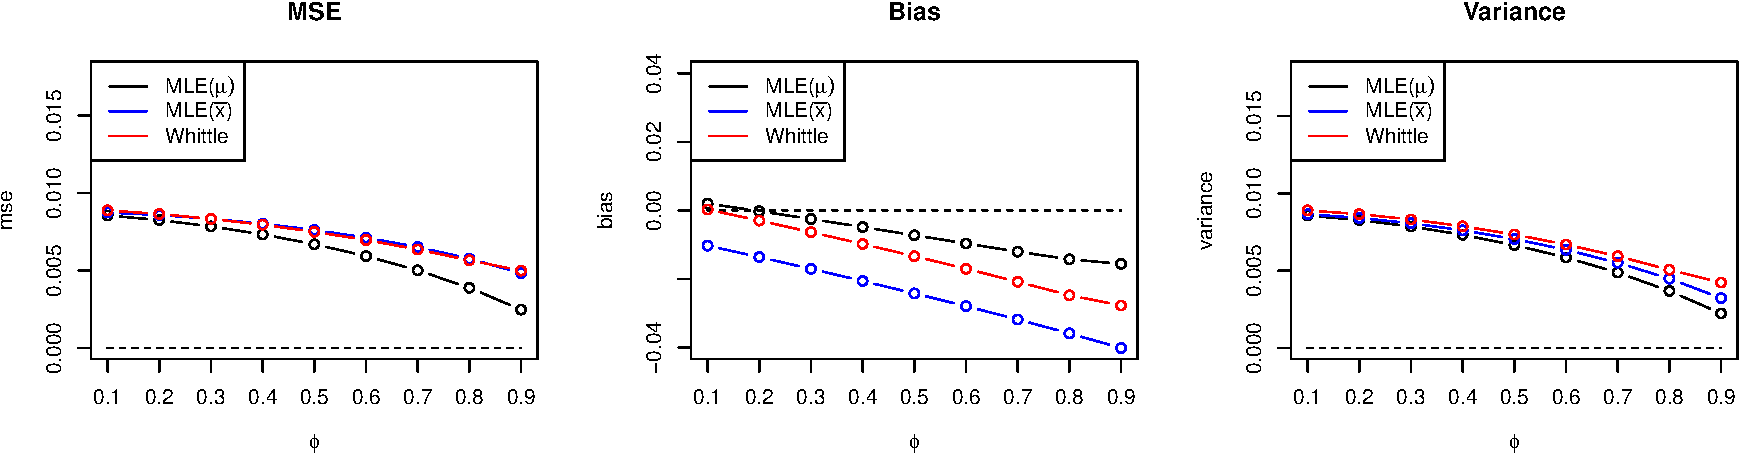
\includegraphics[width=\textwidth]{img/ar1_est_N100.pdf}
		\caption{$n=100$}
	\end{subfigure}
	\begin{subfigure}{\textwidth}
		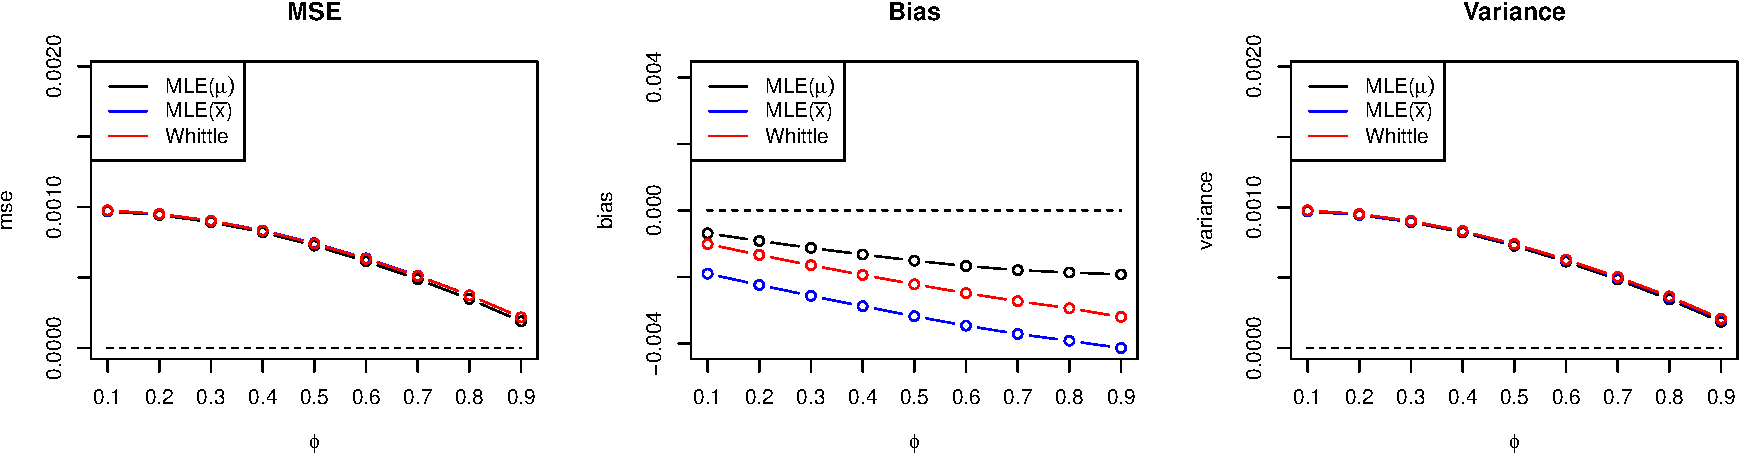
\includegraphics[width=\textwidth]{img/ar1_est_N1000.pdf}
		\caption{$n=1000$}
	\end{subfigure}
	\caption{Среднеквадратичное отклонение, смещение и дисперсия оценок параметра $\phi$ модели $\mathrm{AR}(1)$ ($500$ повторений)}
	\label{tab:ar1_est}
\end{figure}
\begin{figure}[h!]
	\centering
	\begin{subfigure}{\textwidth}
		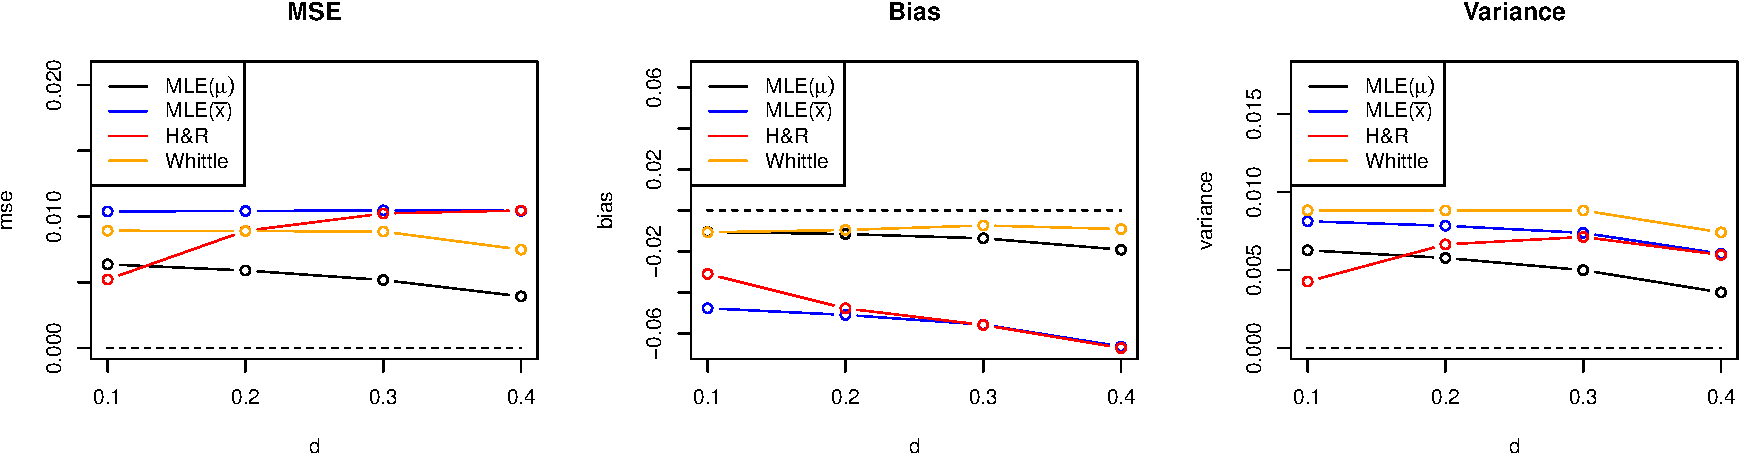
\includegraphics[width=\textwidth]{img/fi_est_N100.pdf}
		\caption{$n=100$}
	\end{subfigure}
	\begin{subfigure}{\textwidth}
		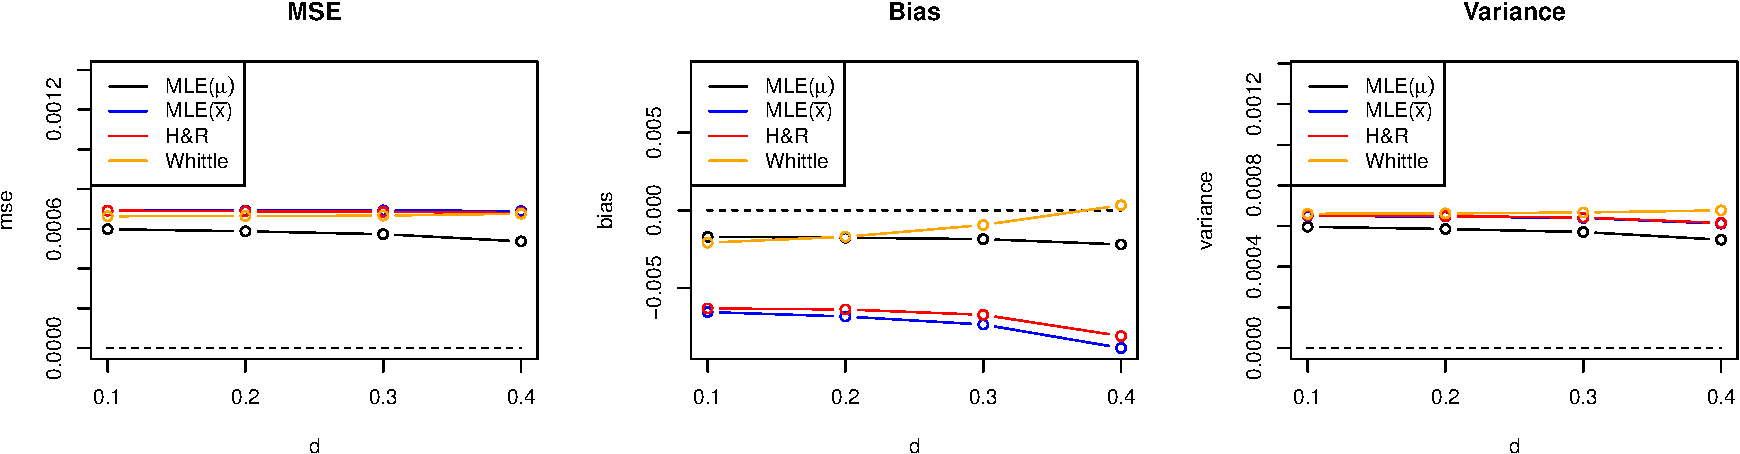
\includegraphics[width=\textwidth]{img/fi_est_N1000.pdf}
		\caption{$n=1000$}
	\end{subfigure}
	\caption{Среднеквадратичное отклонение, смещение и дисперсия оценок параметра $d$ модели $\mathrm{ARFIMA}(0, d, 0)$ ($500$ повторений)}
	\label{tab:fi_est}
\end{figure}

На рис.~\ref{tab:ar1_est} и~\ref{tab:fi_est} изображены среднеквадратичное отклонение, смещение и дисперсия оценок параметров $\phi$ и $d$ моделей $\mathrm{AR}(1)$ и $\mathrm{ARFIMA}(0, d, 0)$. Отметим, что все оценки имеют в большинстве своем отрицательное смещение и отличаются между собой в основном степенью смещения. Как и ожидалось, оценка параметров методом максимального правдоподобия с известным средним дает оценку с наименьшим $\mathsf{MSE}$. С другой стороны, если использовать вместо известного среднего выборочное сренее, оценки становятся сильно смещенными. Whittle же, в свою очередь, дает менее смещенную оценку, чем $\mathrm{MLE}(\bar x)$, а в случае оценки $d$ имеет смещение даже меньше, чем у $\mathrm{MLE}(\mu)$. Однако оценки Whittle обладают наибольшей дисперсией среди всех рассмотренных методов, но разница не такая значительная, как в случае смещения.

\begin{sidewaystable}
	\centering
	\caption{Смещение и среднеквадратичное отклонение оценок параметров $d$ и $\phi$ модели $\mathrm{ARFIMA}(1, d, 0)$ ($n=100$, $500$ повторений)}
	\label{tab:arfi_est}
	\scalebox{0.9}{
	\begin{tabular}{m{1cm}m{1cm}ccccccccm{0.5cm}cccccccc}
		\hline
		& & \multicolumn{8}{c}{$\mathsf{MSE}$} & & \multicolumn{8}{c}{$\mathsf{Bias}$} \\
		\cline{3-10} \cline{12-19}
		& & \multicolumn{2}{c}{$\mathrm{MLE}(\mu)$} & \multicolumn{2}{c}{$\mathrm{MLE}(\bar x)$} & \multicolumn{2}{c}{H\&R} & \multicolumn{2}{c}{Whittle} & & \multicolumn{2}{c}{$\mathrm{MLE}(\mu)$} & \multicolumn{2}{c}{$\mathrm{MLE}(\bar x)$} & \multicolumn{2}{c}{H\&R} & \multicolumn{2}{c}{Whittle} \\
		$d$ &  $\phi$ & $\hat d$ & $\hat\phi$ & $\hat d$ & $\hat\phi$ & $\hat d$ & $\hat\phi$ & $\hat d$ & $\hat\phi$ & & $\hat d$ & $\hat\phi$ & $\hat d$ & $\hat\phi$ & $\hat d$ & $\hat\phi$ & $\hat d$ & $\hat\phi$\\ \hline
		0.1 & 0.1 & 0.071 & 0.075 & 0.205 & 0.179 & \textcolor{blue}{0.009} & \textcolor{red}{0.018} & 0.069 & 0.067 & & -0.096 & 0.083 & -0.301 & 0.26 & \textcolor{blue}{-0.054} & \textcolor{red}{0.035} & -0.086 & 0.068 \\ 
		0.2 & 0.1 & 0.064 & 0.07 & 0.224 & 0.201 & \textcolor{blue}{0.025} & \textcolor{red}{0.032} & 0.077 & 0.073 & & -0.095 & 0.083 & -0.336 & 0.296 & -0.119 & 0.099 & \textcolor{blue}{-0.094} & \textcolor{red}{0.074} \\ 
		0.3 & 0.1 & 0.081 & 0.086 & 0.303 & 0.272 & \textcolor{blue}{0.049} & \textcolor{red}{0.055} & 0.084 & 0.081 & & -0.12 & 0.108 & -0.427 & 0.386 & -0.179 & 0.161 & \textcolor{blue}{-0.109} & \textcolor{red}{0.09} \\ 
		0.4 & 0.1 & \textcolor{blue}{0.072} & \textcolor{red}{0.08} & 0.367 & 0.328 & 0.081 & 0.089 & 0.179 & 0.194 & & \textcolor{blue}{-0.119} & \textcolor{red}{0.111} & -0.499 & 0.456 & -0.243 & 0.23 & -0.26 & 0.241 \\
		\hline
		0.1 & 0.5 & 0.057 & 0.048 & 0.099 & 0.059 & \textcolor{blue}{0.01} & \textcolor{red}{0.015} & 0.057 & 0.054 & & -0.102 & 0.065 & -0.258 & 0.185 & -0.07 & 0.033 & \textcolor{blue}{-0.066} & \textcolor{red}{0.024} \\ 
		0.2 & 0.5 & 0.055 & 0.045 & 0.107 & 0.062 & \textcolor{blue}{0.031} & \textcolor{red}{0.025} & 0.074 & 0.058 & & \textcolor{blue}{-0.108} & \textcolor{red}{0.071} & -0.277 & 0.201 & -0.154 & 0.108 & -0.153 & 0.107 \\ 
		0.3 & 0.5 & \textcolor{blue}{0.051} & \textcolor{red}{0.041} & 0.119 & 0.068 & 0.063 & 0.043 & 0.098 & 0.062 & & \textcolor{blue}{-0.114} & \textcolor{red}{0.079} & -0.304 & 0.225 & -0.232 & 0.174 & -0.209 & 0.161 \\ 
		0.4 & 0.5 & \textcolor{blue}{0.052} & \textcolor{red}{0.043} & 0.129 & 0.074 & 0.104 & 0.065 & 0.104 & 0.066 & & \textcolor{blue}{-0.131} & \textcolor{red}{0.098} & -0.326 & 0.244 & -0.306 & 0.235 & -0.228 & 0.177 \\ 
		\hline
		0.1 & 0.9 & 0.029 & 0.028 & 0.013 & 0.008 & \textcolor{blue}{0.007} & \textcolor{red}{0.007} & 0.034 & 0.025 & & 0.07 & -0.085 & 0.003 & -0.044 & \textcolor{blue}{0.001} & \textcolor{red}{-0.043} & 0.049 & -0.069 \\ 
		0.2 & 0.9 & 0.019 & 0.021 & 0.011 & 0.006 & \textcolor{blue}{0.009} & \textcolor{red}{0.004} & 0.026 & 0.019 & & 0.038 & -0.063 & \textcolor{blue}{-0.013} & -0.034 & -0.037 & \textcolor{red}{-0.026} & 0.02 & -0.056 \\ 
		0.3 & 0.9 & 0.013 & 0.016 & \textcolor{blue}{0.009} & 0.004 & 0.014 & \textcolor{red}{0.003} & 0.022 & 0.015 & & \textcolor{blue}{0.007} & -0.043 & -0.033 & -0.022 & -0.076 & \textcolor{red}{-0.011} & -0.024 & -0.039 \\ 
		0.4 & 0.9 & \textcolor{blue}{0.009} & 0.018 & \textcolor{blue}{0.009} & 0.004 & 0.025 & \textcolor{red}{0.002} & 0.028 & 0.01 & & \textcolor{blue}{-0.019} & -0.036 & -0.059 & -0.011 & -0.121 & \textcolor{red}{0.003} & -0.095 & -0.016 \\ 
		\hline
	\end{tabular}
	}
\end{sidewaystable}

В таблице~\ref{tab:arfi_est} представлены значения среднеквадратичной ошибки и смещения оценок параметров $d$ и $\phi$ модели $\mathrm{ARFIMA}(1, d)$. Заметим, что в оценках присутствует смещение, и оно уменьшается с увеличением $\phi$. Также для $\phi=0.1$ и $\phi=0.5$ оценки $d$ имеют отрицательное смещение, а оценки $\phi$, наоборот, положительное. Также в таблице синим цветом выделена лучшая по строке оценка $d$, а красным --- лучшая оценка $\phi$. Видно, что метод H\&R в большинстве случаев дает оценки с наименьшим $\mathsf{MSE}$, однако оценки имеют большое смещение при $\phi=0.1$ и $\phi=0.5$. Наиболее смещенные оценки получаются в методе $\mathrm{MLE}(\bar x)$, причем это перестает быть таковым только при $\phi=0.9$. Оценки методом Whittle по смещению находятся посередине, однако имеют наибольшую дисперсию среди остальных. 
% \begin{table}[h!]
% 	\centering
% 	\caption{Смещение и среднеквадратичное отклонение оценок параметра $\phi$ модели $\mathrm{AR}(1)$ ($n=100$, $500$ повторений)}
% 	\begin{tabular}{m{1cm}cccm{0.5cm}ccc}
% 		\hline
% 		& \multicolumn{3}{c}{$\mathsf{bias}\cdot 100$} & & \multicolumn{3}{c}{$\mathsf{MSE}\cdot 100$} \\
% 		\cline{2-4} \cline{6-8}
% 		$\phi$ & $\mathrm{MLE}(\mu)$ & $\mathrm{MLE}(\bar x)$ & Whittle & & $\mathrm{MLE}(\mu)$ & $\mathrm{MLE}(\bar x)$ & Whittle \\ \hline
% 		0.1 & 0.197  & -1.029 &  0.025 & & 0.856 & 0.874 & 0.889\\
% 		0.2 & -0.023 & -1.362 & -0.298 & & 0.826 & 0.859 & 0.865\\
% 		0.3 & -0.252 & -1.707 & -0.635 & & 0.785 & 0.834 & 0.834\\
% 		0.4 & -0.487 & -2.061 & -0.981 & & 0.733 & 0.802 & 0.796\\
% 		0.5 & -0.725 & -2.423 & -1.337 & & 0.670 & 0.762 & 0.75\\
% 		0.6 & -0.965 & -2.796 & -1.704 & & 0.594 & 0.712 & 0.697\\
% 		0.7 & -1.205 & -3.183 & -2.084 & & 0.502 & 0.652 & 0.636\\
% 		0.8 & -1.427 & -3.59  & -2.478 & & 0.389 & 0.577 & 0.566\\
% 		0.9 & -1.560 & -4.016 & -2.777 & & 0.248 & 0.483 & 0.5\\
% 		\hline
% 	\end{tabular}
% \end{table}

\bibliographystyle{ugost2008}
\bibliography{report}

\end{document}
